\documentclass[10pt, aspectratio=169]{beamer}
\usepackage[utf8]{inputenc}
\usepackage[T1]{fontenc}
\usepackage{tikz-cd}
\usepackage{latexsym}
\usepackage{amsmath}
\usepackage{amsfonts}
\usepackage[mathcal]{eucal}
\usepackage{adjustbox}
\usepackage{xspace}
\usepackage{amsthm}
\usepackage{hyperref}
\usepackage[french]{babel}
\hypersetup{
    colorlinks=true,
    linkcolor=.,
    filecolor=magenta,      
    urlcolor=cyan,
}

\usepackage{graphicx}
\usepackage{pgf}
\usepackage{pgfpages}
\usepackage[outputdir=cache,cache=false]{minted}
\usetheme{metropolis}           % Use metropolis theme
\newcommand{\norm}[1]{\left\Vert #1 \right\Vert}
\newcommand{\expect}[1]{\mathop{\mathbb{E}}_{#1}}
\newcommand{\alertbf}[1]{\textbf{\alert{#1}}}
\title{\emph{Présentation de ...} \\ \emph{One-bit Compressed Sensing by Linear Programming}\\ Yaniv Plan \& Roman Vershynin (CPAM, 2013)}
\date{11 mars 2021}
\author{Théodor Lemerle \& Théophile Cantelobre \\ 
Master M2A -- Sorbonne Université}
\begin{document}
  \maketitle
  
  \begin{frame}{Sommaire}
  \tableofcontents{}
  \end{frame}
  
  \section{Motivation}
  \begin{frame}[t]{Motivation: traitement du signal \& CS idéal}
 \begin{figure}
     \centering
     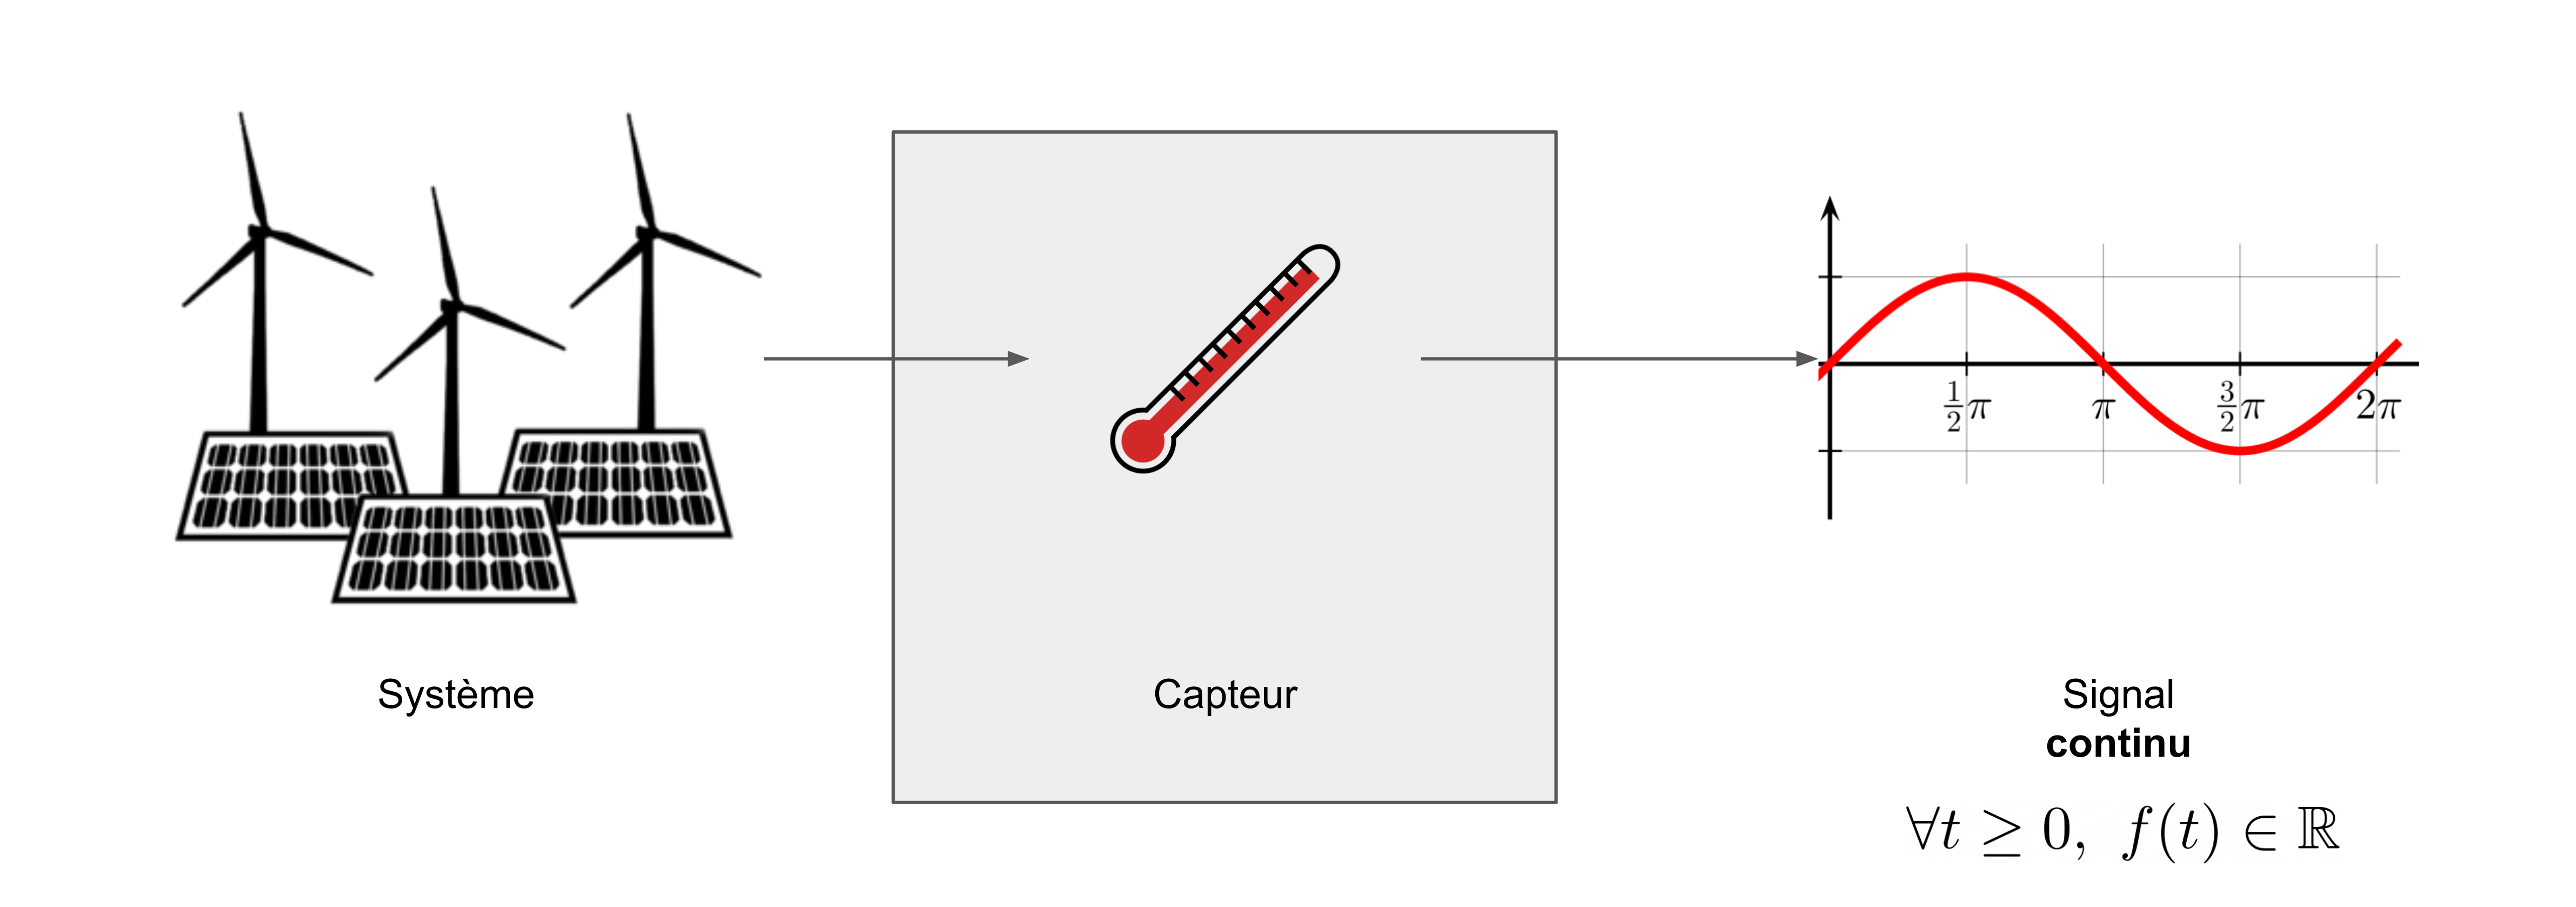
\includegraphics[width=0.8\textwidth]{figures/continous.png}
 \end{figure} 
  \begin{itemize}
      \item CS permet de reconstruire complètement le signal à partir de mesures... sans atteindre la fréquence de Nyquist-Shannon.
      \item Hypothèse: $f(t)\in\mathbb{R}$... précision infinie !
  \end{itemize}
  \end{frame}
  
  \begin{frame}[t]{Motivation: traitement du signal \& CS avec quantization}
 \begin{figure}
     \centering
     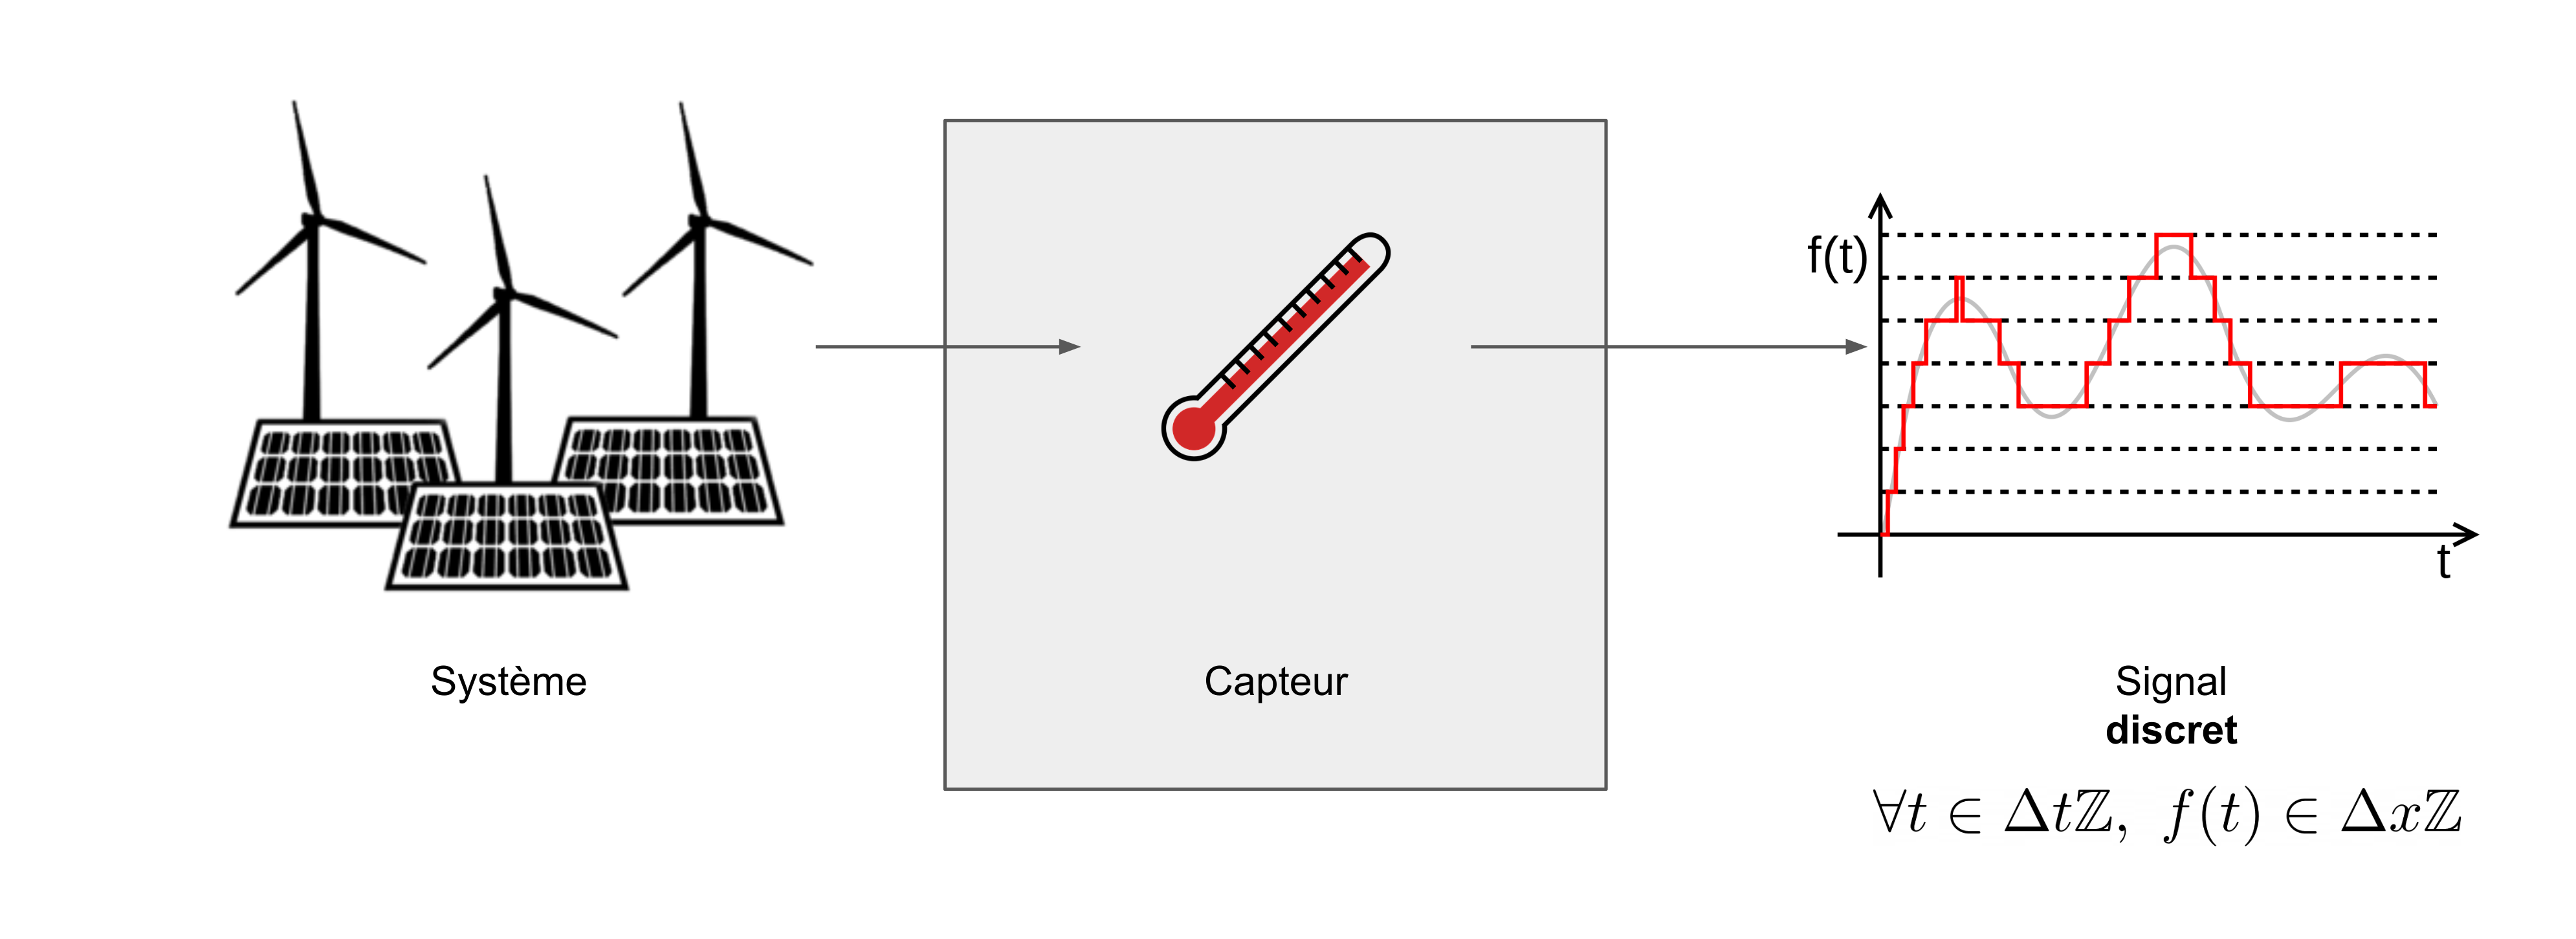
\includegraphics[width=0.8\textwidth]{figures/discrete.png}
 \end{figure} 
  \begin{itemize}
      \item Quantization comme bruit: CS permet de le corriger !
      \item Deux approches pour traiter le bruit de discrétisation: même nombre de bits !
      \begin{itemize}
          \item Augmenter le nombre de bits par mesure: hardware lent.
          \item Augmenter le nombre de mesures: hardware rapide.
      \end{itemize}
  \end{itemize}
  \end{frame}

  \begin{frame}[t]{Quantization extrême: 1-bit compressed sensing}
    Poussé à l'extrême: \textbf{mesures avec 1-bit} (signes).
   
   \begin{block}{Perte de l'amplitude}
\smallskip
   $$\forall \lambda >0, ~\mathrm{sign}(A\lambda x) = \mathrm{sign}\left(Ax\right)$$
   \end{block} 
   
   \begin{block}{Problème de dégénérescence $(\mathcal B \mathcal P)$}
\smallskip
   \begin{align}
       \min_{x\in\mathbb R^n}{}& \norm{x}_1 \\
       \mathrm{s.t.} & ~~\mathrm{sign}(Ax)=y 
   \end{align}
   ...decrease objective by multiplying admissible iterate by $\lambda \rightarrow 0^+$.
   \end{block} 
  \end{frame}
 \section{Garanties théoriques} 
  \begin{frame}[t]{Principal résultat}
    \begin{theorem}[Théorème 1.1]
        Soient $n$, $m$, et $s >0$. Soit A une \textbf{matrice gaussienne} de taille $m\times n$. Soit $\delta >0$ dépendant de $s$, $m$ et $n$. Alors, avec une probabilité au moins $1 - C\exp(-c \delta m)$, on a \textbf{uniformément} sur tout $x\in\mathbb R^n$ qui sont \textbf{essentiellement parcimonieux} d'ordre $s$: si $ y = \mathrm{sign}(Ax)$. Alors, la solution $\hat x$ du problème $(\mathcal P_{1-bit})$ vérifie:
        $$\left\Vert \frac{\hat x}{\Vert \hat x\Vert_2} - \frac{x}{\Vert x\Vert_2}\right\Vert_2 \leq \delta.$$
    \end{theorem} 
    
    \begin{block}{Situation par rapport au cours}
\smallskip
    
    \begin{table}[ht]
        \centering
        \begin{tabular}{c|c}
             Points communs &  Différences\\
             \hline
             Garanties uniformes. &  Essentiellement parcimonieux.\\
        Matrice de mesure gaussienne. & Reconstruction \emph{inexacte}.
        \end{tabular}
    \end{table}
    \end{block}
  \end{frame}
  
  \begin{frame}{Remarque: essentiellement parcimonieux}
  \begin{block}{Essentiellement parcimonieux}
\smallskip
  $$ ES(x) = \frac{\Vert x\Vert_1^2}{\Vert x\Vert_2^2} \leq s$$
  \end{block}
\begin{block}{Expérience numérique}
\smallskip
\begin{columns}
  \begin{column}{0.45\textwidth}
  Pour des vecteurs $s$-parcimonieux aléatoires, $ES(x)$ estime bien $\norm{x}_0$ :
  $$0.6 s \lessapprox ES(x) \lessapprox{0.75} s $$
  \end{column}
  \begin{column}{0.45\textwidth}
\begin{figure}
    \centering
    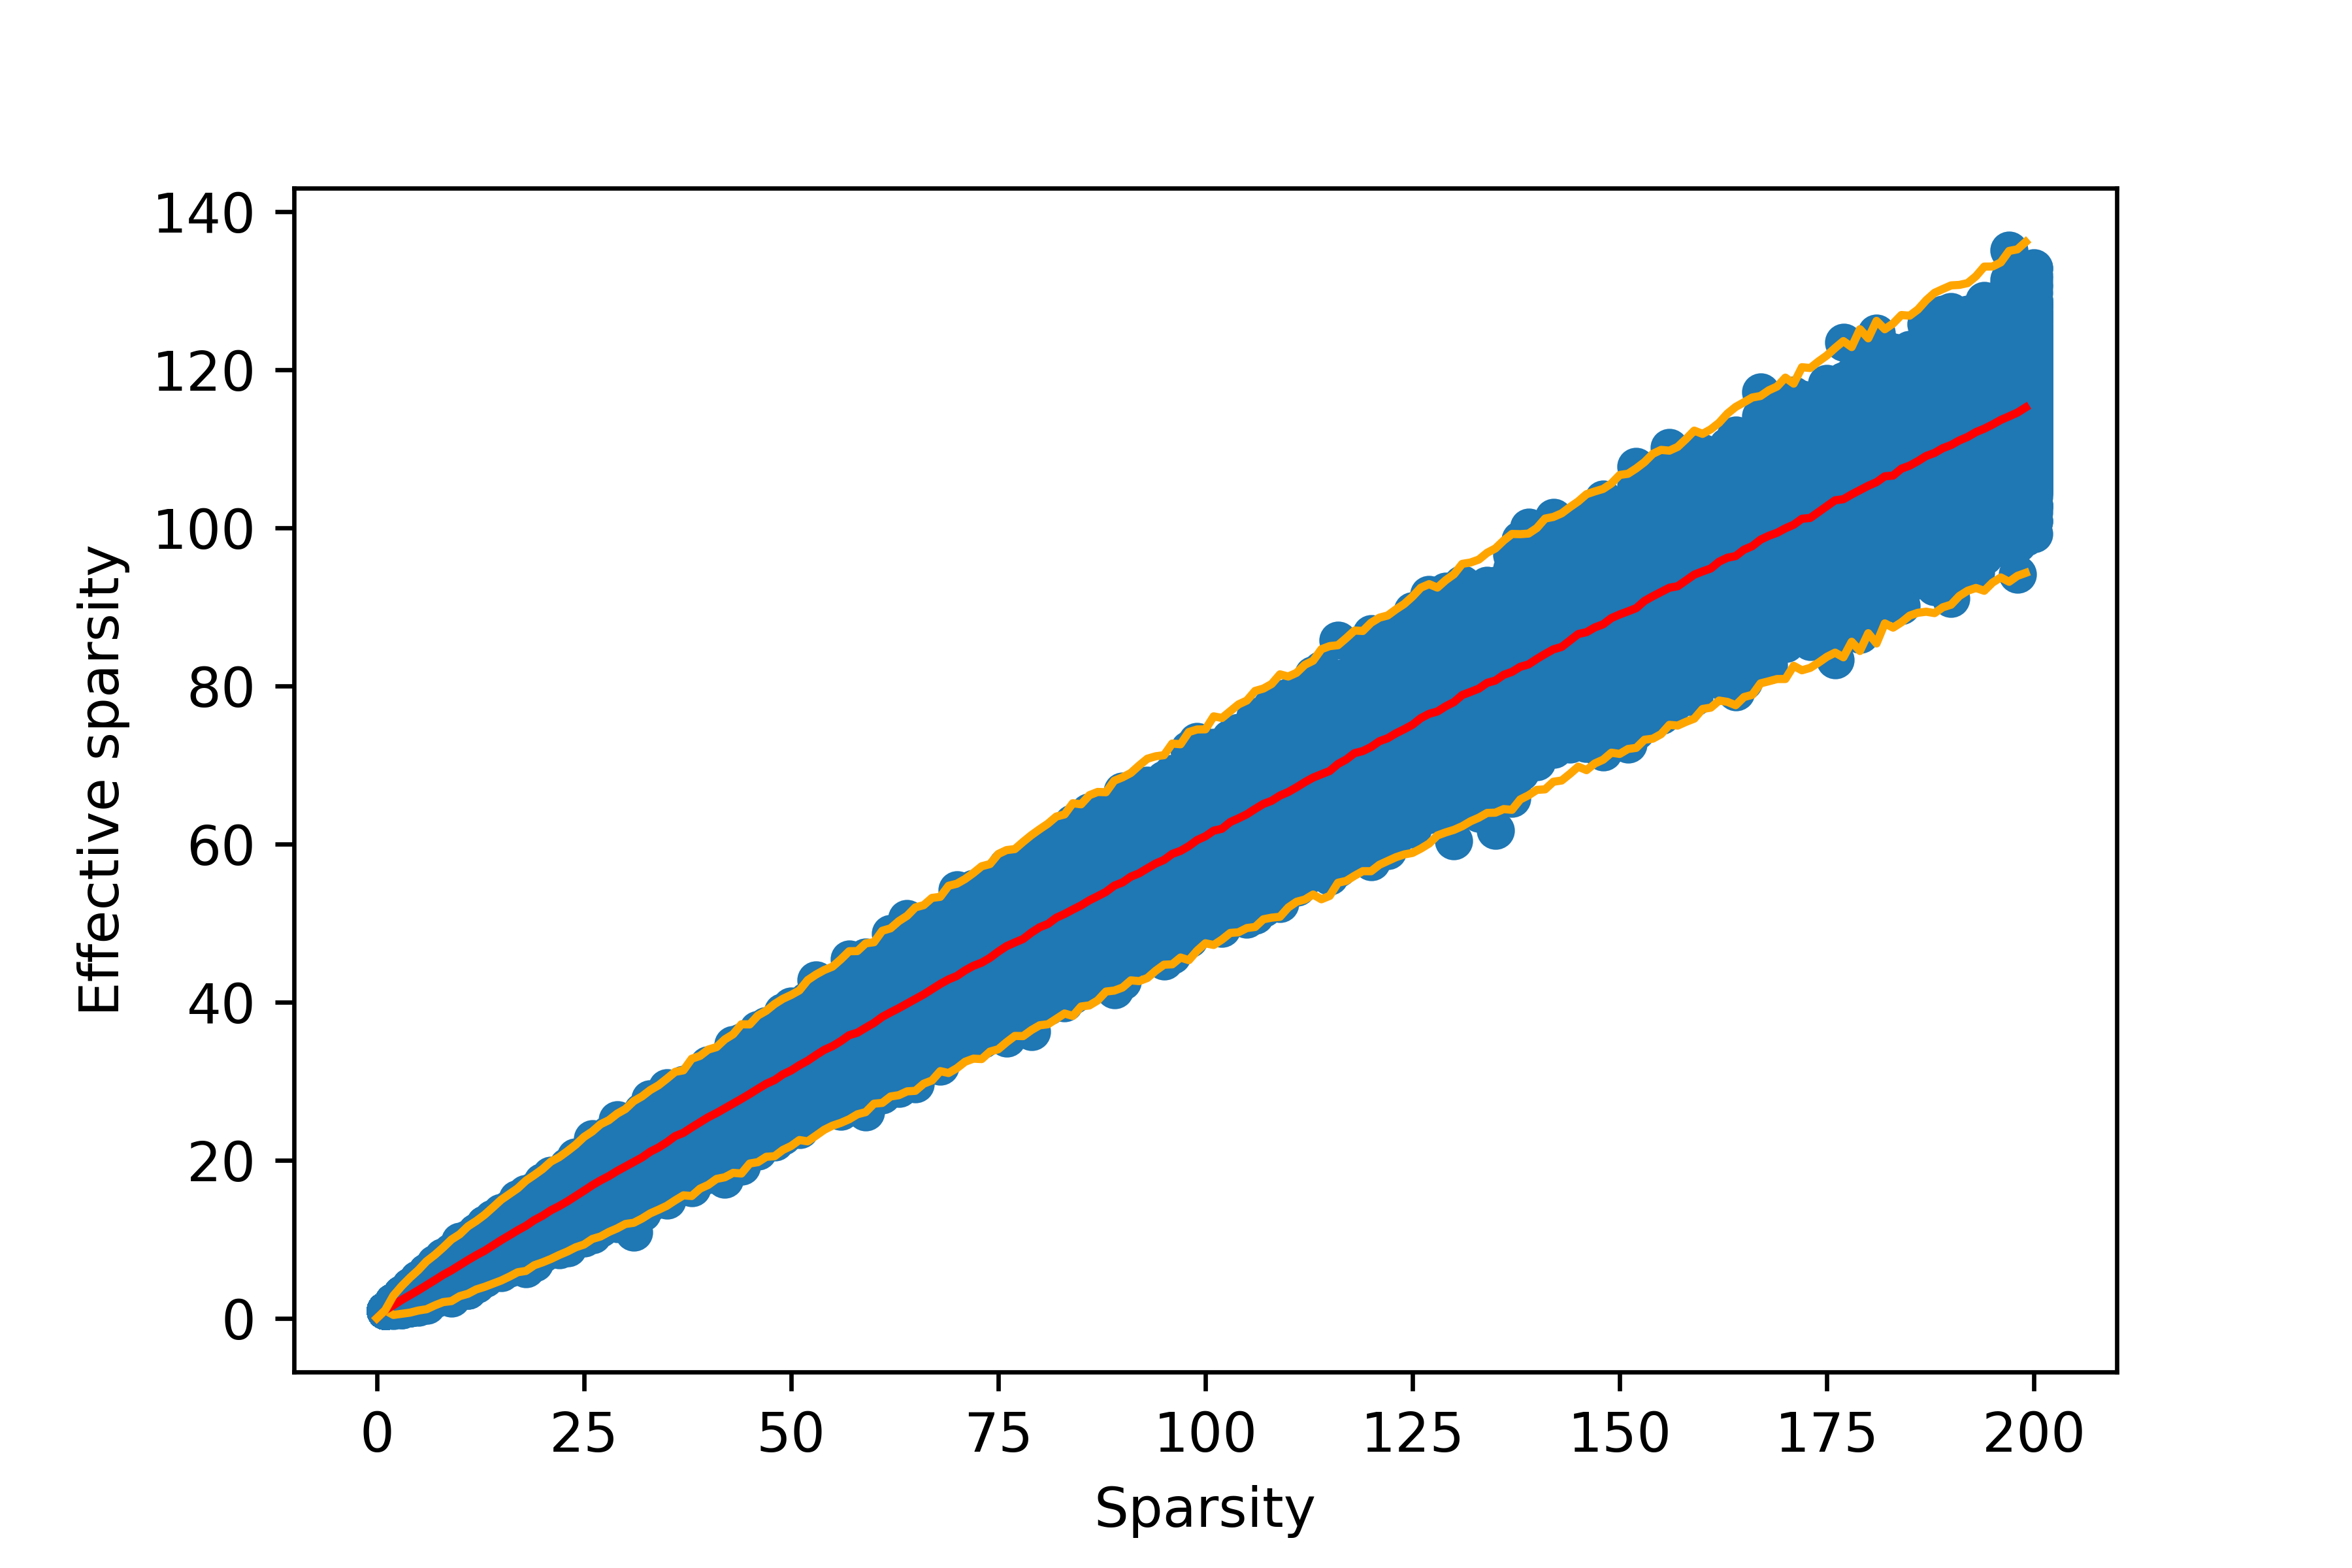
\includegraphics[width=0.90\textwidth]{figures/es.png}
\end{figure}    
  \end{column}
\end{columns}
     
    \end{block} 
  \end{frame}

\begin{frame}{Stratégie de la preuve}
\begin{block}{1. Géométrie de la reconstruction à partir du signe.}
\smallskip
        \textbf{Outils principaux:} random tesselations \& $\varepsilon$-nets.
        
        \textbf{Résultat objectif:} pour $m$ bien choisi, w.h.p. si $\mathrm{sign}(Ax)=\mathrm{sign}(Ax^\prime)$ alors $\norm{x-x^\prime}_2 \leq \delta$.
\end{block}
\begin{block}{2. Vecteurs essentiellement parcimonieux}
\smallskip
        \textbf{Outils principaux:} concentration de la mesure.
        
        \textbf{Résultat objectif:} Une solution de notre problème d'optimisation préserve la parcimonie essentielle du signal d'intérêt : $$ES(\hat{x}) \leq  ES(x) \cdot C \sqrt{\log(2n/m + 2m/n)}  $$
\end{block}

\begin{block}{$\rightarrow$ Mise en commun}
\smallskip
$\hat x$ vérifie 2, donc 1 tient pour $x$ et $\hat x$ en particulier.
\end{block}
\end{frame}

\begin{frame}{Esquisse de la preuve: partie 1/2}
\begin{block}{Idée générale}
\smallskip
\centering
Quantifier combien de mesures gaussiennes de 1-bit il faut pour séparer tous les signaux possibles:\\

\textbf{avec h.p. uniformément sur les $x,y$, si $\norm{x-y}_2 > \delta$, il existe $\Omega(m)$ hyperplans qui séparent $x$ et $y$.}
\end{block}
\begin{block}{1. Contrôles des têtes et des queues}
\smallskip
\begin{enumerate}
    \item Séparer $x$ (et $y$) en: $x=\underbrace{x_0}_\text{$\in$ net}+ \varepsilon x^\prime$.
    \item S'assurer que les $x_0$ et $y_0$ sont séparés par $\Omega(m)$ hyperplans.
    \item S'assurer que les $x^\prime$ et $y^\prime$ le sont par $\Omega(m) - o(m)$ hyperplans.
    \item Tout mettre ensemble.
\end{enumerate}
\end{block}
\begin{block}{2. Plus petit $\varepsilon$-net possible.}

$$ \log N(K_{n,s}, \varepsilon) \leq \frac{Cs}{\varepsilon^2} \log \left(\frac{2n}{s}\right)$$
\end{block}
 
\end{frame}
\begin{frame}{Esquisse de la preuve: partie 2/2}
\smallskip
On veut montrer : $\frac{\Vert \hat{x}\Vert_2^2}{\Vert \hat{x}\Vert_1^2} \leq  \frac{\Vert {x}\Vert_2^2}{\Vert {x}\Vert_1^2} \cdot C \sqrt{\log(2n/m + 2m/n)}  $

\begin{block}{Un résultat de concentration uniforme sur la déviation moyenne.}
$$\frac{1}{m} \norm{Ax}_1 \geq \frac{\norm{x}_2}{2} \text{avec proba. au moins } 1-C \exp(-cm) $$\\
La preuve reprend les grandes idées de la preuve de la propriété RIP pour les matrices à entrées gaussiennes.
\end{block}
\begin{block}{Une borne inférieure sur $\norm{\hat{x}}_2$}
$$ \norm{\hat{x}}_2 \geq c/ \sqrt{\log(2n/m + 2m/n)}$$
\end{block}
Mis bout à bout :
$$\frac{\norm{\hat{x}}_1}{\norm{\hat{x}}_2} \leq \frac{\norm{x}_1}{\norm{Ax}_1 \norm{\hat{x}}_2} \leq  \frac{2\norm{x}_1}{\norm{\hat{x}}_2 \norm{x}_2} \leq \frac{\Vert {x}\Vert_2^2}{\Vert {x}\Vert_1^2} \cdot C \sqrt{\log(2n/m + 2m/n)} $$
\begin{block}{}

\end{block}
\end{frame}

\begin{frame}{Résumé: un programme linéaire (LP) à résoudre}
\smallskip
\begin{columns}
    \begin{column}{0.45\textwidth}
   \begin{align*}
       \min_{x\in\mathbb R^n}{}& \norm{x}_1 \\
       \mathrm{s.t.} & ~~\mathrm{sign}(Ax)=y \\
       & ~~ \norm{Ax}_1\geq m 
   \end{align*}
    \end{column}
    \pause
    \begin{column}{0.45\textwidth}
   \begin{align*}
       \min_{u\in\mathbb R^n}{}& \mathbf{1}^T u \\
       \mathrm{s.t.}& ~~ \forall i, ~-u_i \leq y_i \leq u_i\\
       & ~~\forall i, ~u_i \geq 0\\
       & ~~\forall i, ~y_i\langle A_i, x\rangle=1\\
       & ~~ \langle y, Ax\rangle\geq m 
   \end{align*}
    \end{column}
\end{columns}
    
\end{frame}


\section{Expériences}
\begin{frame}{Méthodologie expérimentale}
\begin{block}{Protocole expérimental}
\smallskip
\begin{enumerate}
    \item Générer un signal parcimonieux (dans une certaine base): $x$.
    \item Tirer une matrice $A\sim \mathcal N(0, 1)$.
    \item Observer $y=\mathrm{sign}(Ax)$.
    \item Résoudre $(\mathcal P_{1-bit})$: $\hat x$.
\end{enumerate}
... répéter $N_{trials}$ fois.
    
\end{block}
\pause
\begin{block}{Métriques: comment évaluer une reconstruction? voir [18]}
\smallskip
\begin{itemize}
\item Erreur angulaire: $\epsilon(x, \hat x) = \frac{1}{\pi}\arccos \langle x, \hat x \rangle$
\item Signal-to-Noise ratio: $\mathrm{SNR}(x, \hat x) = 20 \log_{10} \frac{\Vert x\Vert_2}{\Vert x - \hat x\Vert_2}$
\item (Distance de Hamming: $d_H(y, \hat y) = \frac{1}{m}\sum_{i=1}^m \mathrm{XOR}(\mathrm{sign}(Ay),\mathrm{sign}(A\hat y))$)
\end{itemize}
\end{block}
\end{frame}

\begin{frame}{Méthodes comparées: Basis pursuit, BIHT... and 1-bit LP}
\begin{block}{Basis pursuit (avec seuillage)}
\smallskip
Programmation linéaire puis seuillage:
   \begin{align*}
       \min_{x\in\mathbb R^n}{}& \norm{x}_1 \\
       \mathrm{s.t.} & ~~ Ax=y 
   \end{align*}
\end{block}
\begin{block}{Binary Iterative Hard Thresholding [18]}
\smallskip
Descente de gradient projetée (pour $\norm{\cdot}_0$ = Hard Thresholding ) :
    \begin{align*}
        \min_{x\in\mathbb R^n}{}& \frac{1}{2} \norm{y - Ax}_2^2\\
               \mathrm{s.t.} & ~~ \norm{x}_0 = s
    \end{align*}
\end{block}
\end{frame}
\begin{frame}{Reconstruction de signaux parcimonieux synthétiques (1/2)}
\begin{figure}
    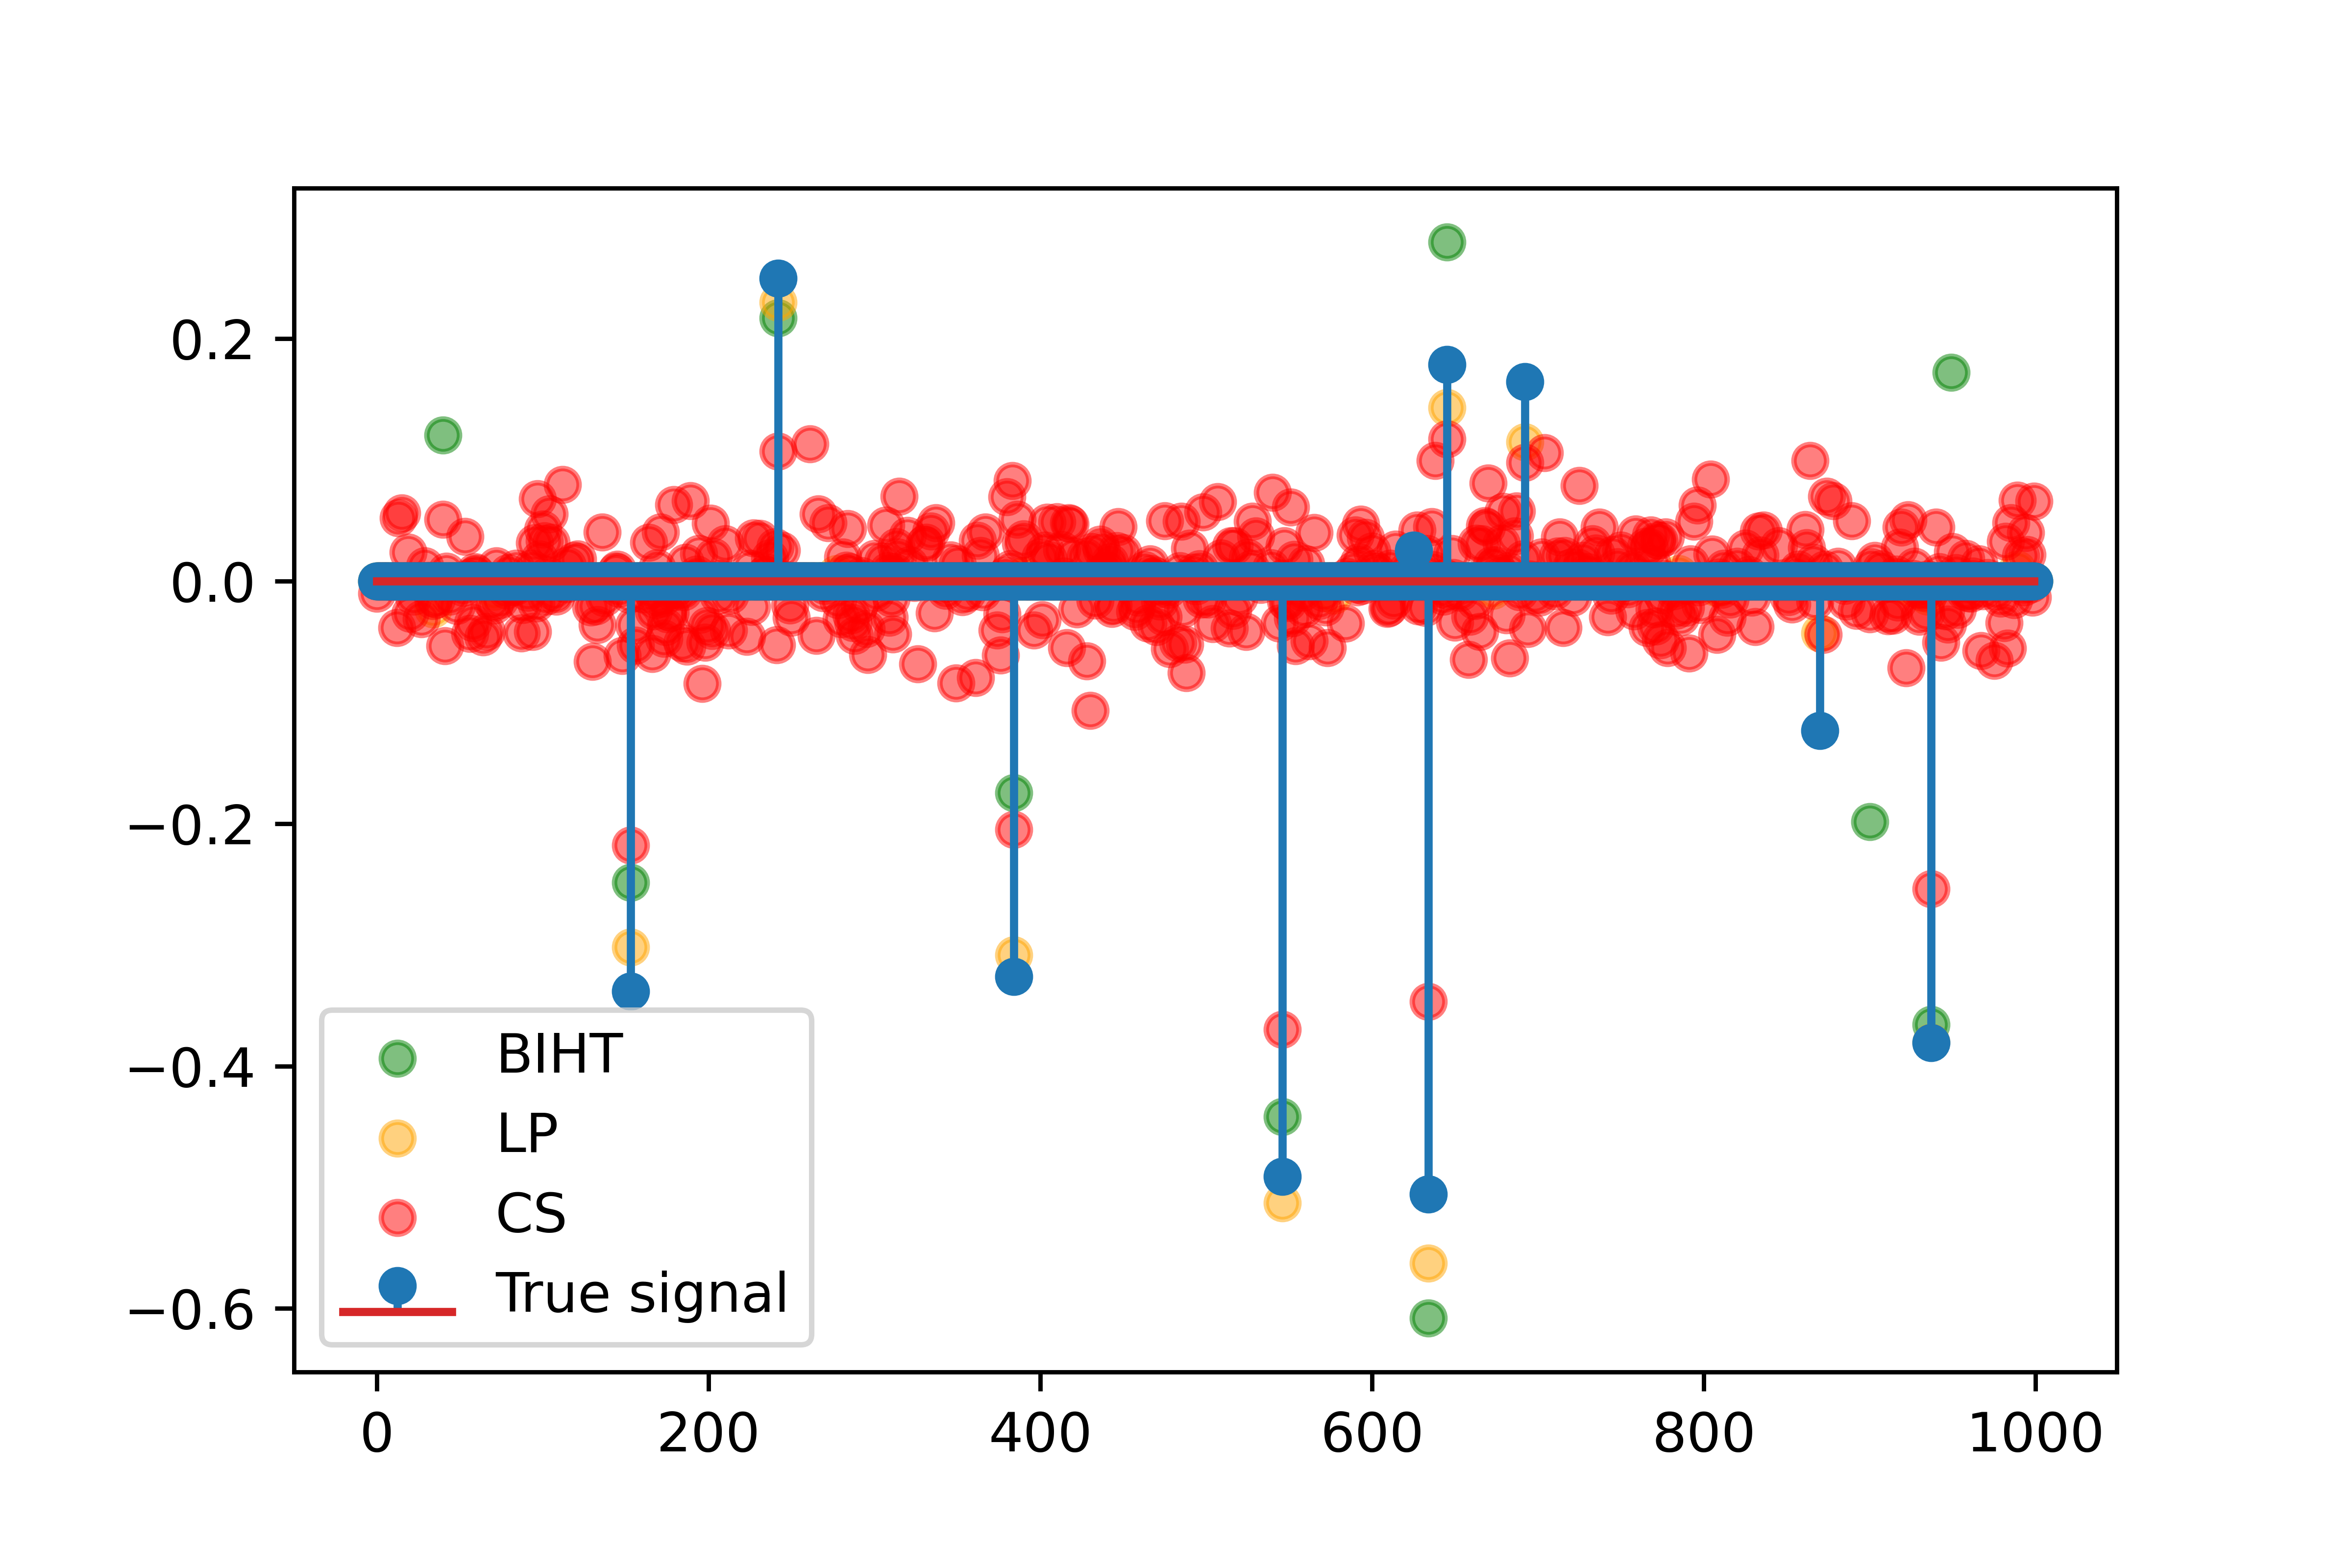
\includegraphics[width=0.5\textwidth]{figures/recon-synth-500.png}%
    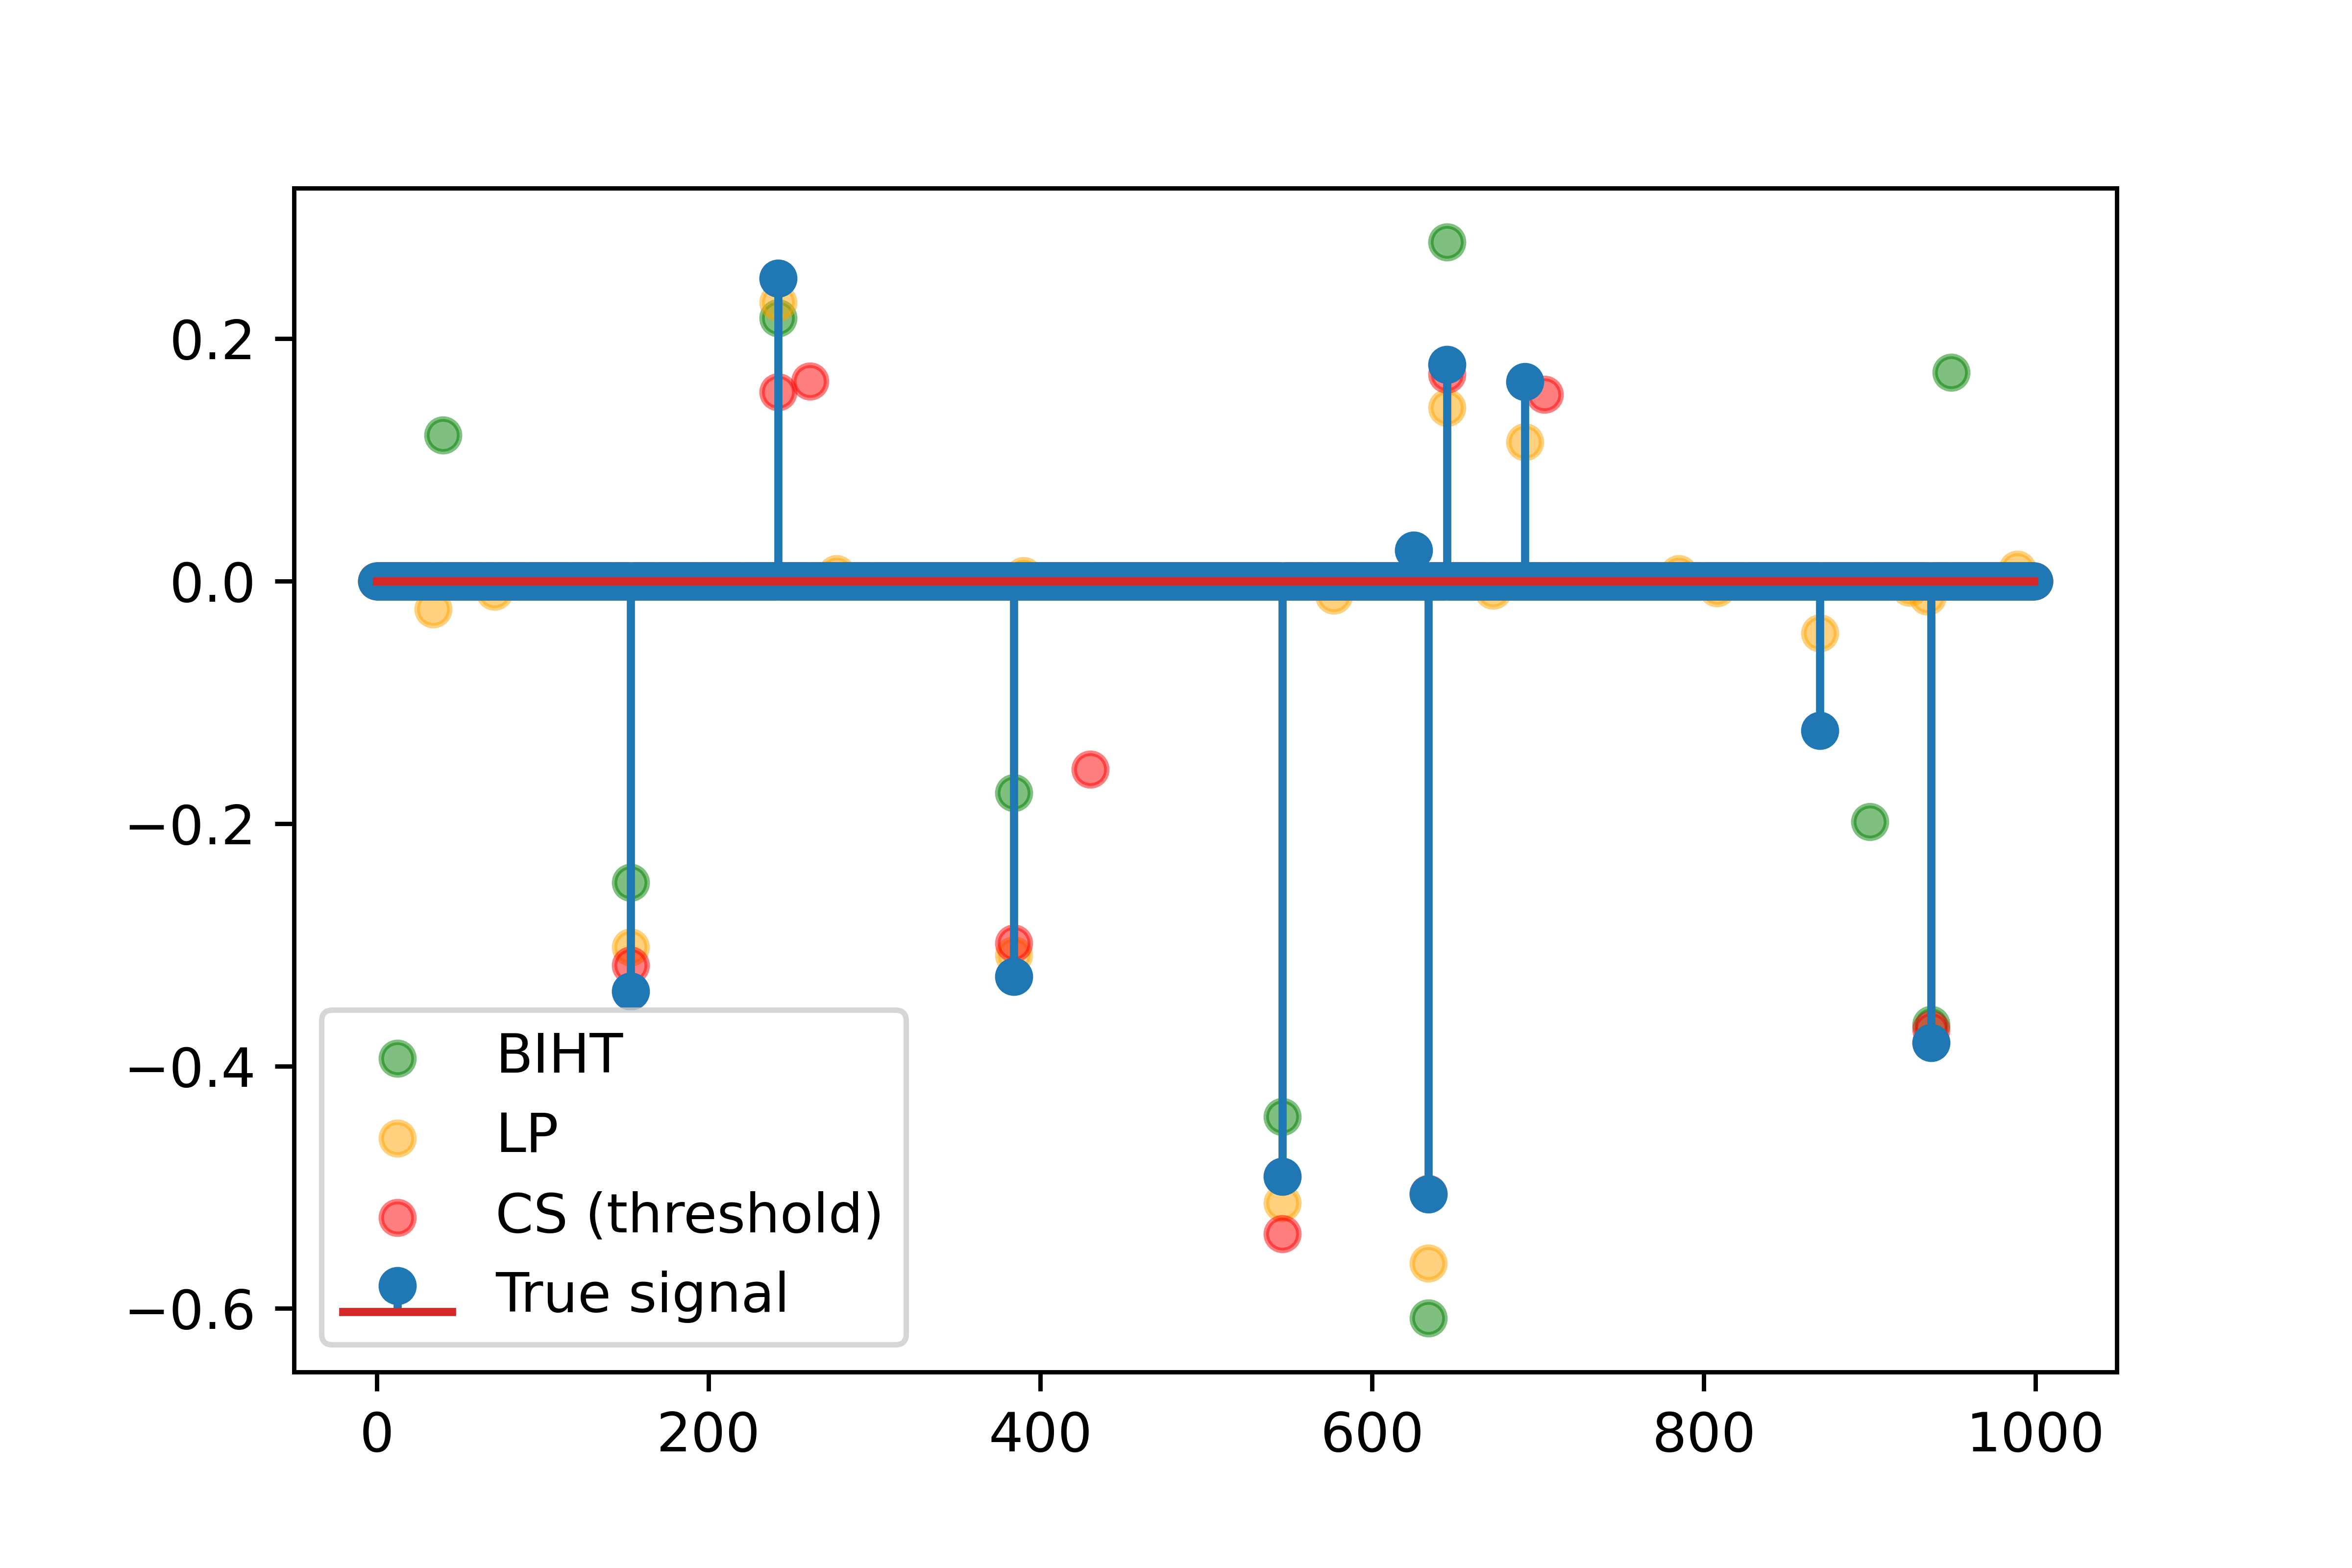
\includegraphics[width=0.5\textwidth]{figures/recon-synth-500-thresh.png}
\end{figure}    
\end{frame}

\begin{frame}{Reconstruction de signaux parcimonieux synthétiques (2/2)}
\begin{figure}
    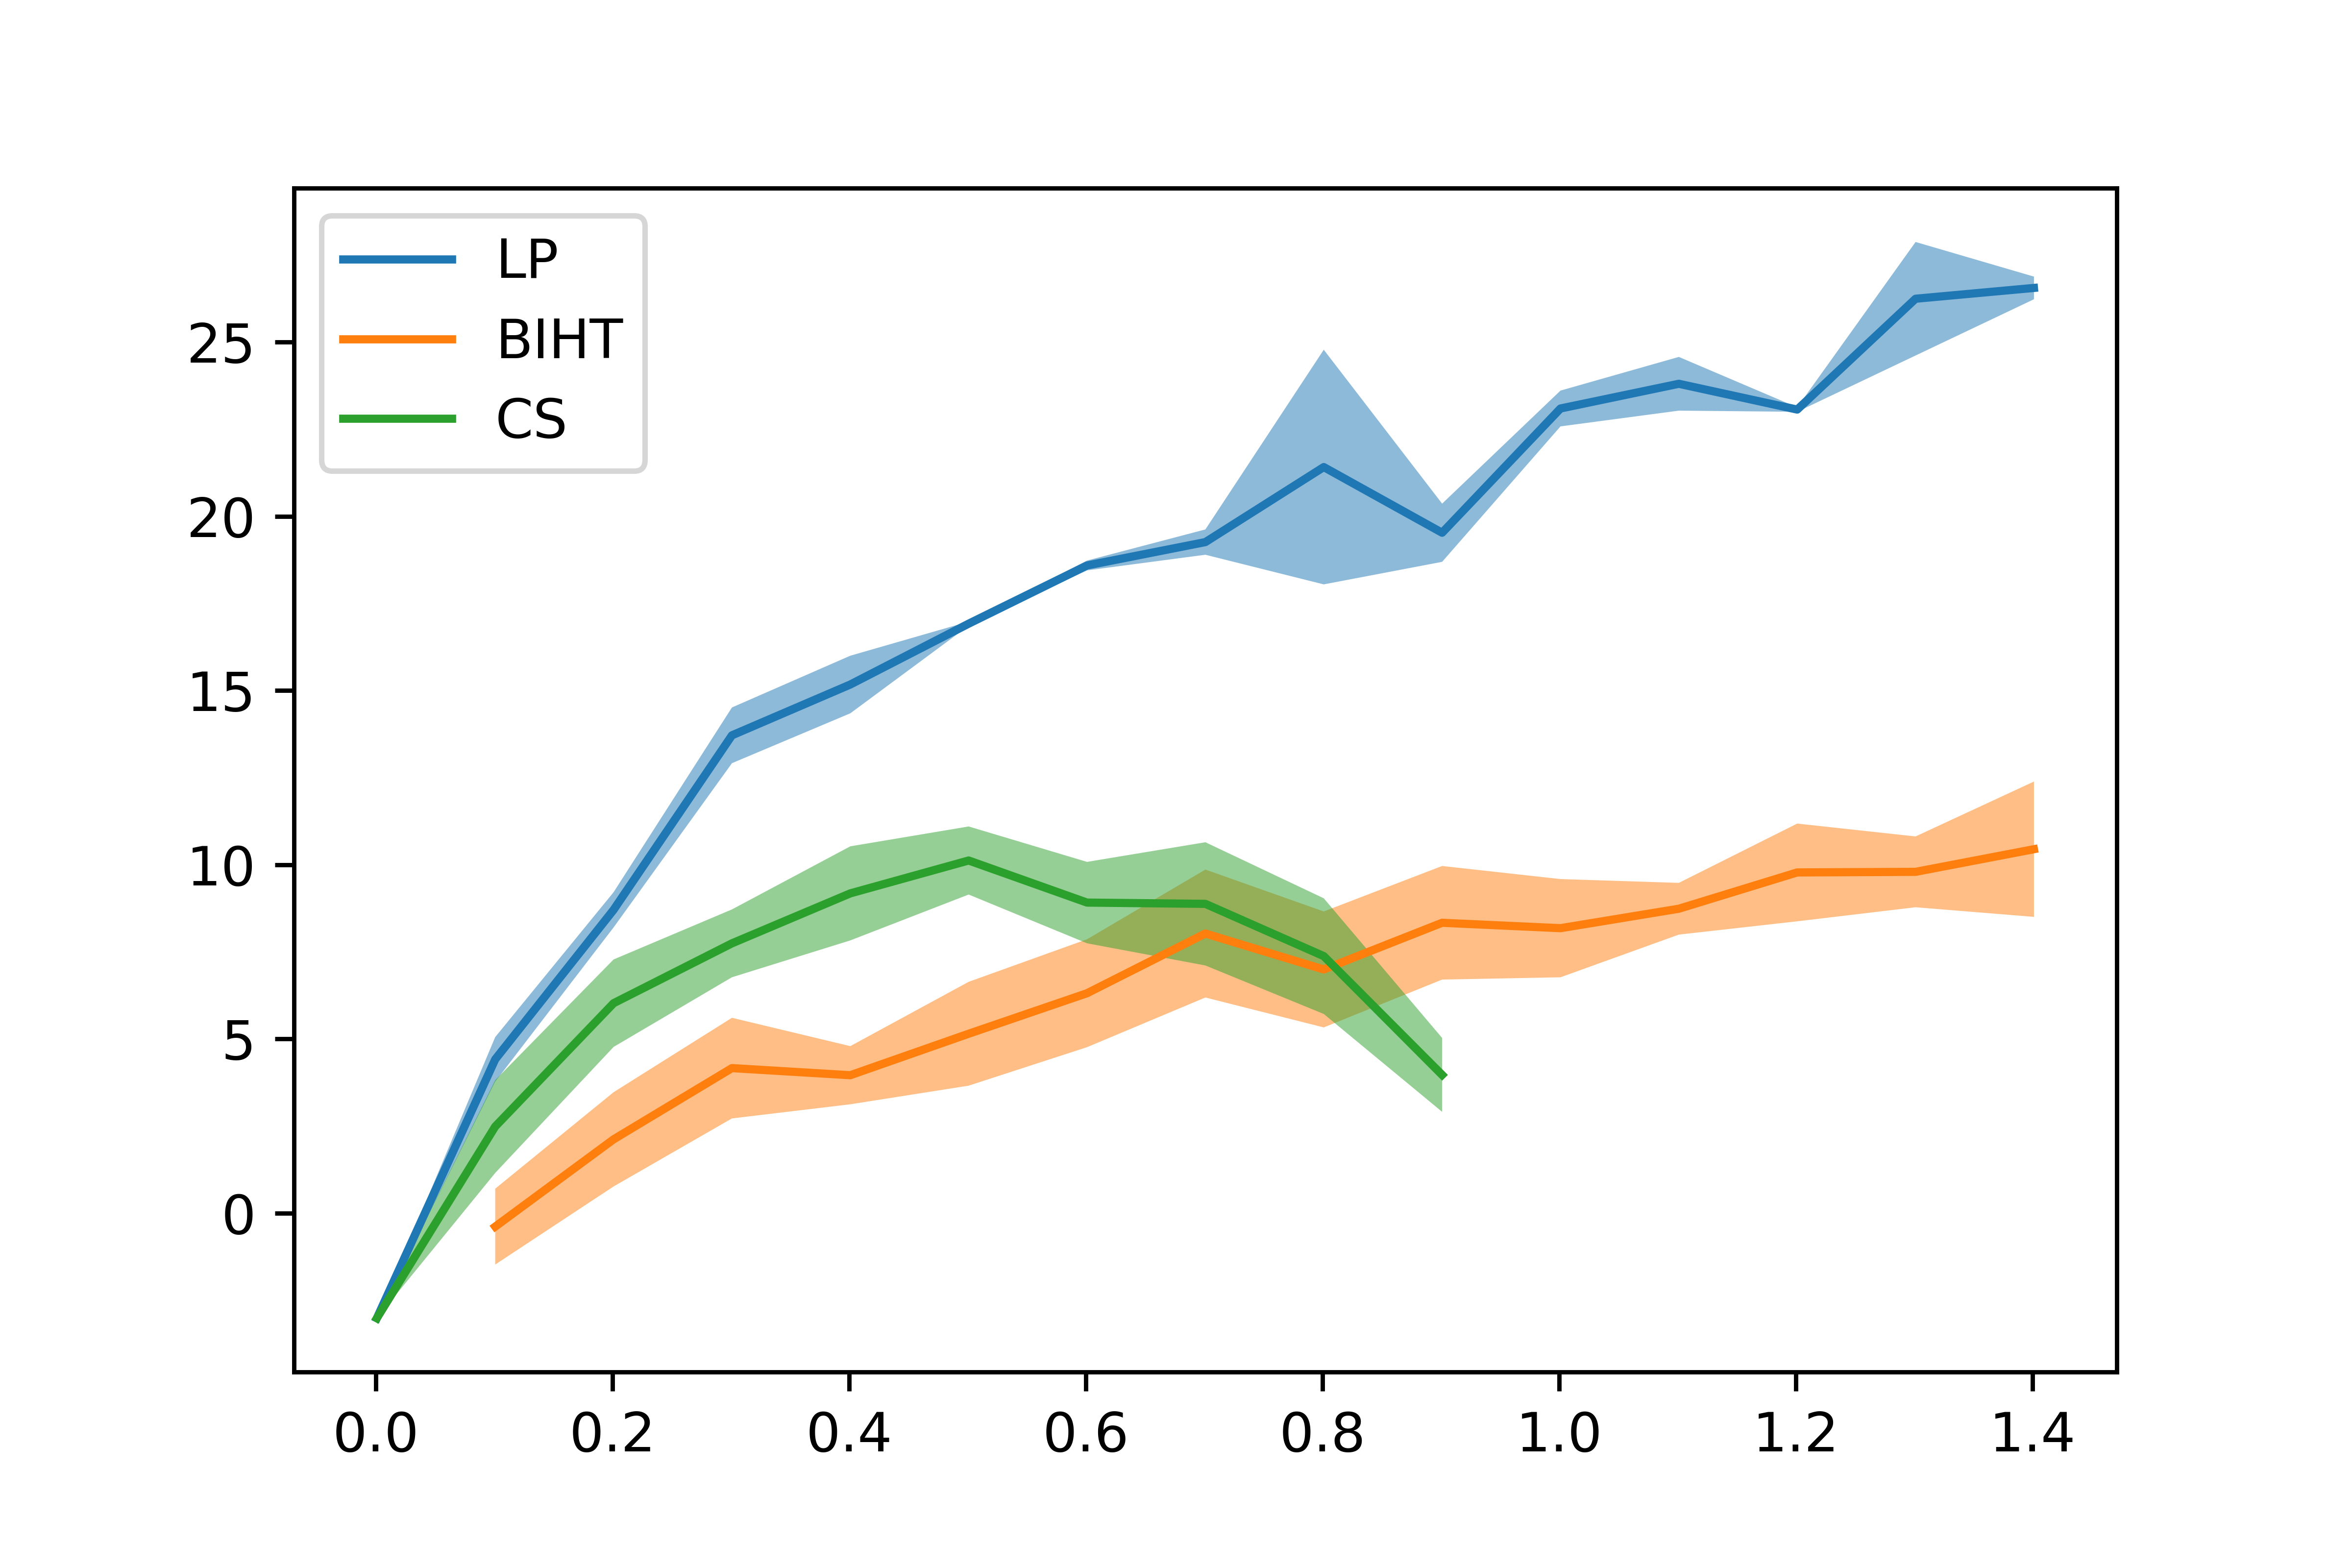
\includegraphics[width=0.5\textwidth]{figures/summary_snr.png}%
    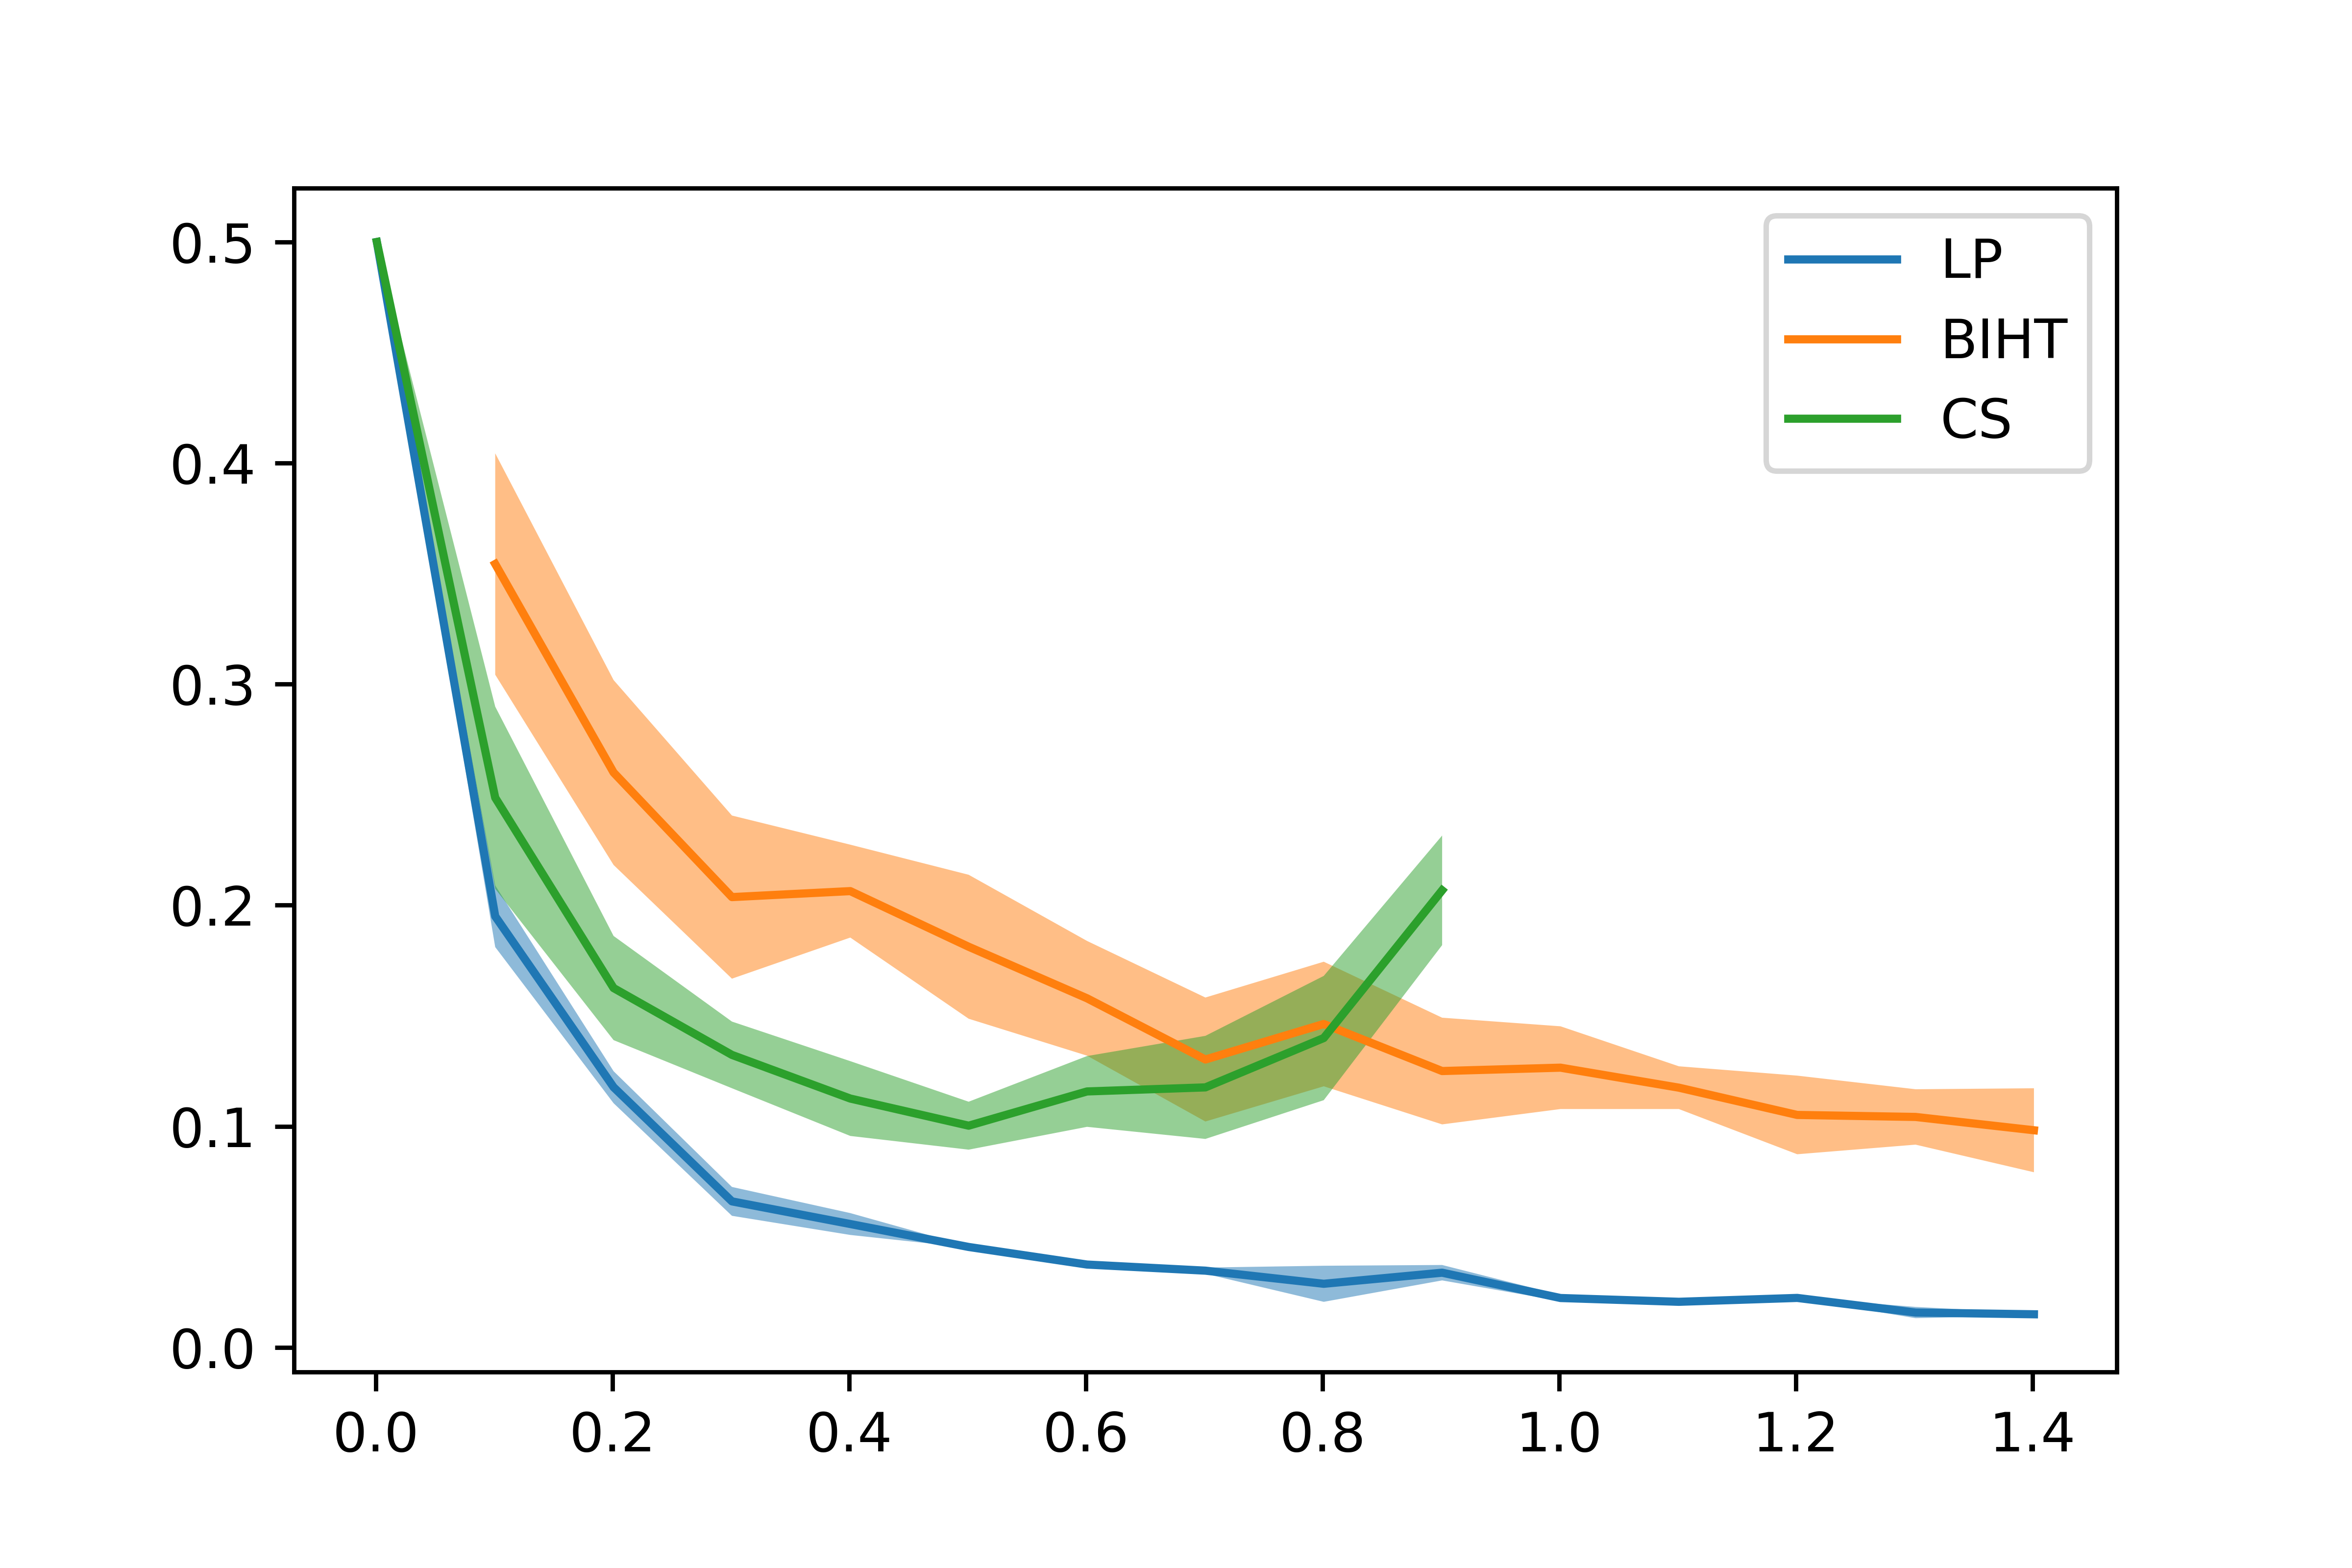
\includegraphics[width=0.5\textwidth]{figures/summary_angular.png}
\end{figure}    
\centering
Performance moyenne (10 essais) avec écart type. \\À gauche: $\mathrm{SNR}$. À droite: erreur angulaire. En abscisse: $m/n$.
\end{frame}
\begin{frame}{Eye candy: \texttt{MNIST}}
\begin{figure}
    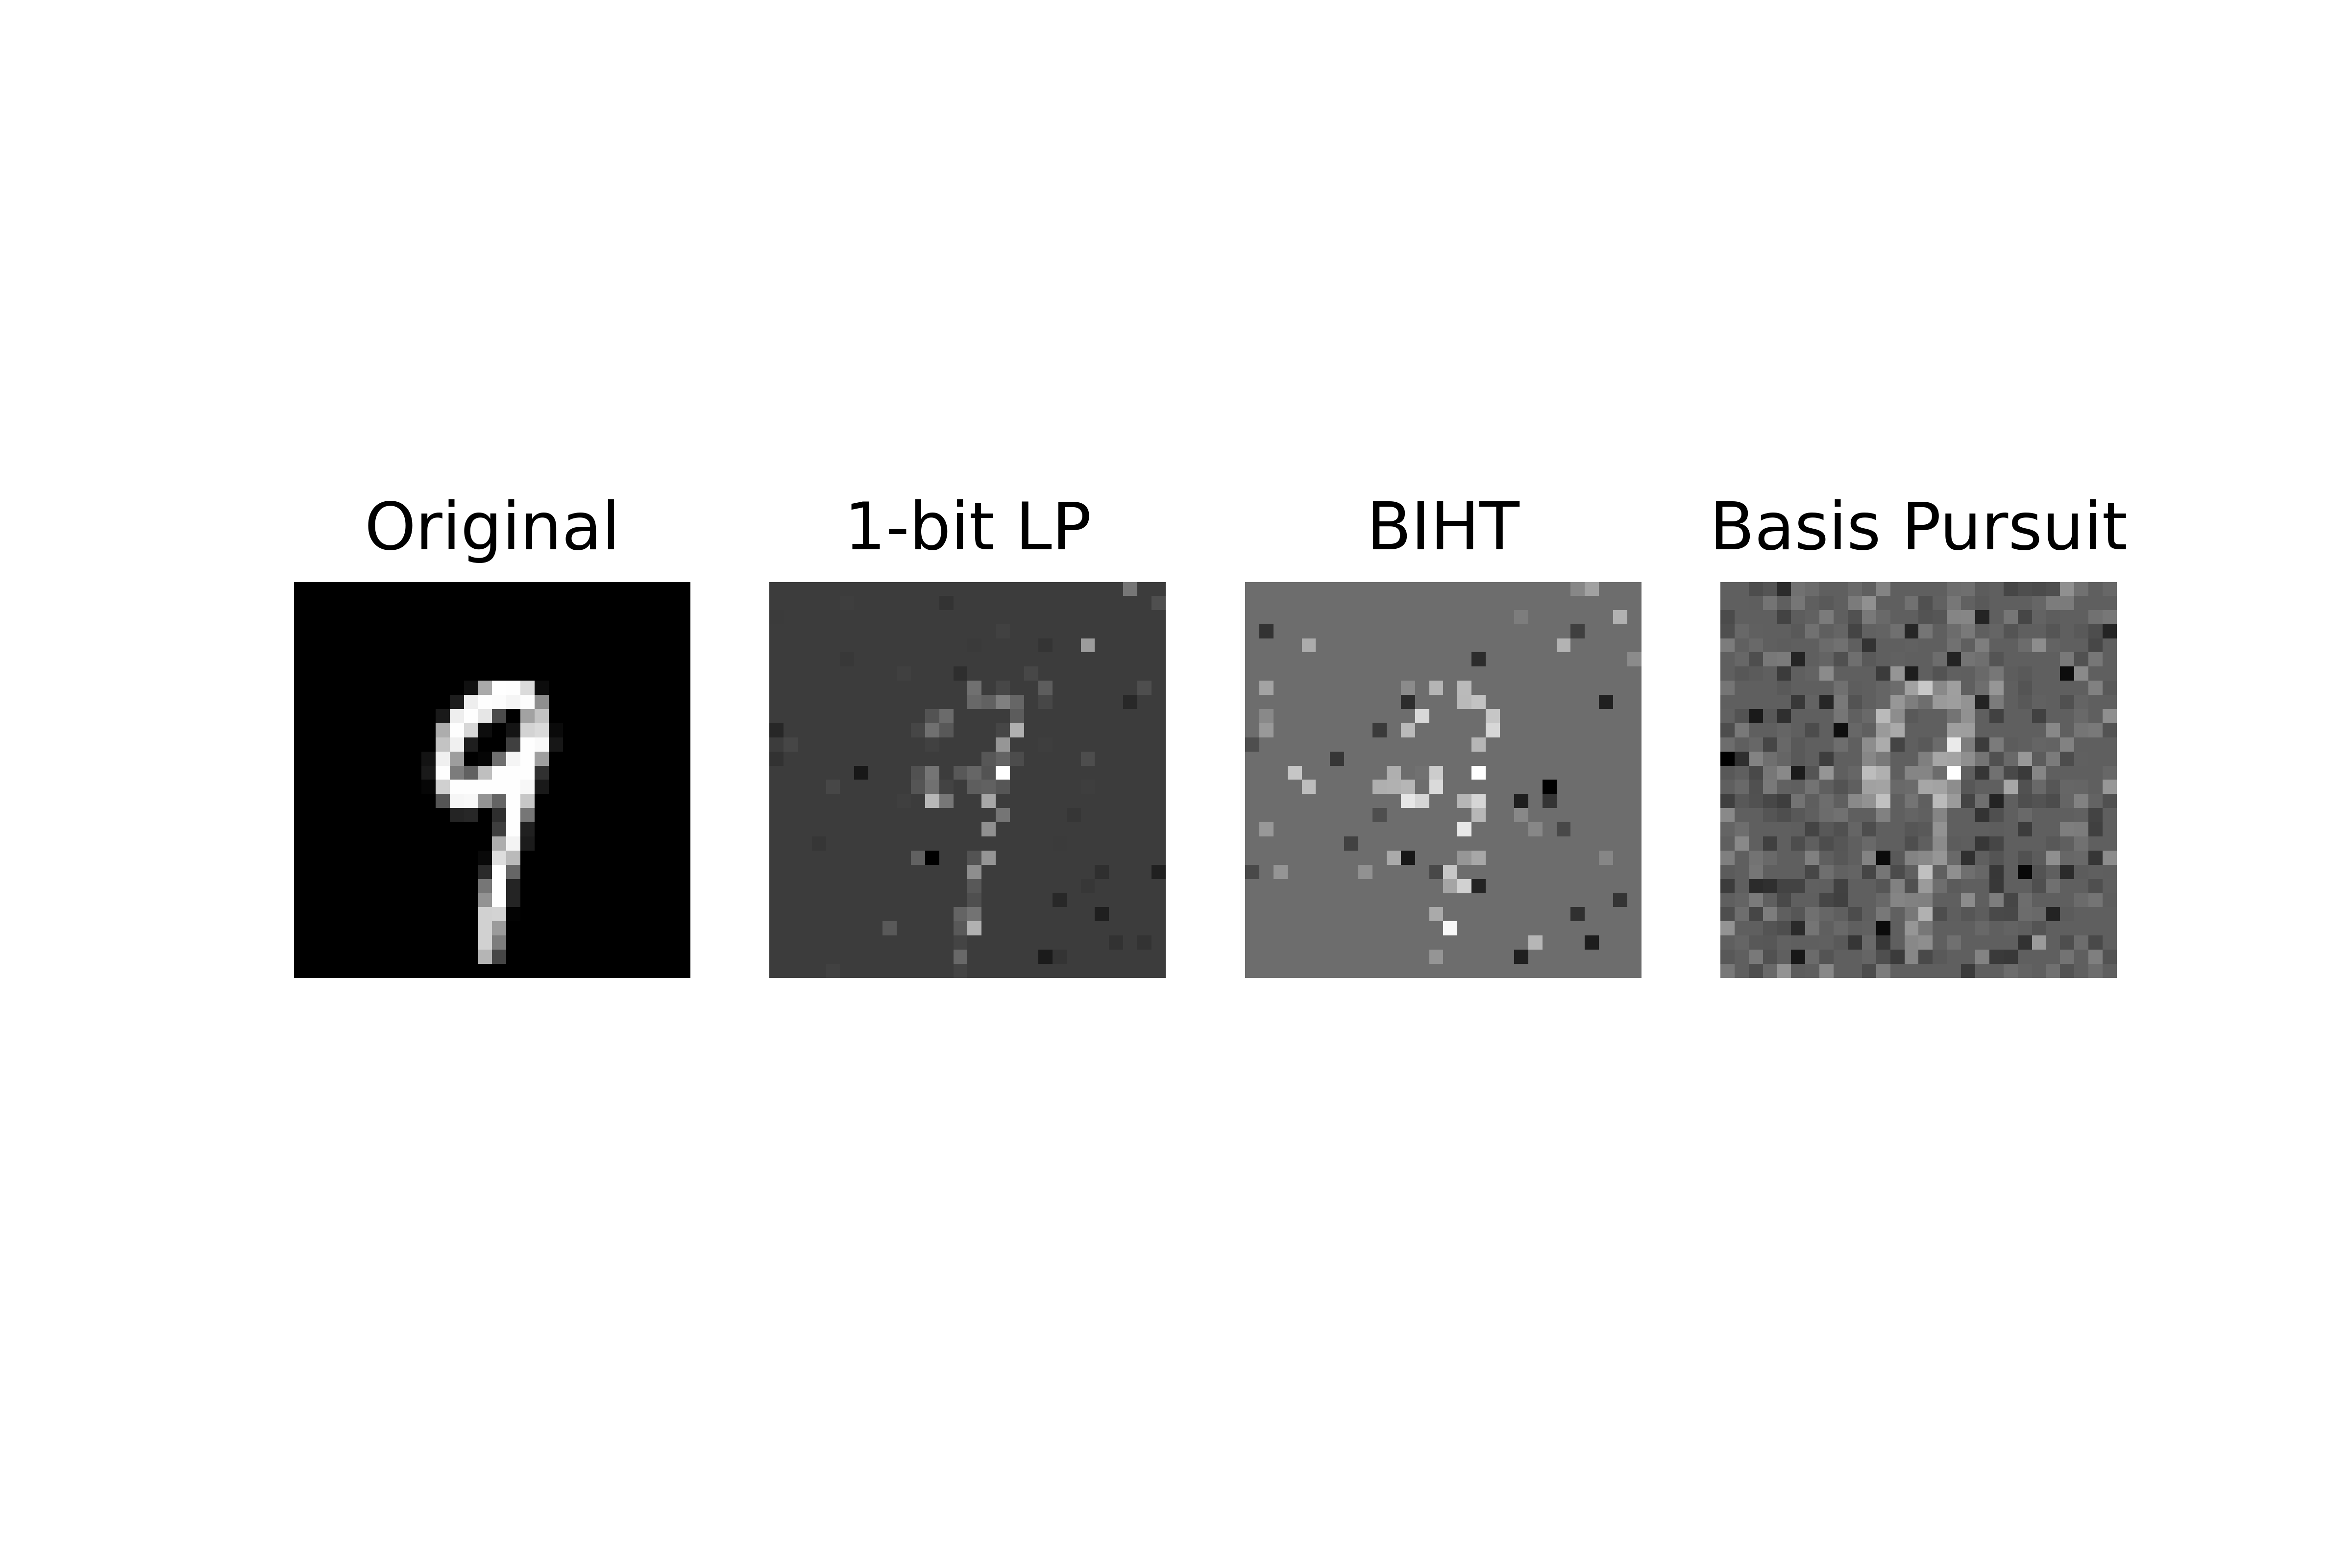
\includegraphics[width=1\textwidth]{figures/mnist.png}%
\end{figure}    
\end{frame}

\section{Résumé \& Conclusion}

\begin{frame}{Résumé \& Conclusion}

\begin{block}{1-bit compressed sensing with LP}
\smallskip

\begin{itemize}
    \item Reconstruction approximative du signal d'intérêt sur $\mathbb{S}^{n-1}$.
    \item Garanties uniformes sur les signaux essentiellement parcimonieux ($\Sigma_s \subset K_{n,s}$).
    \item Programme linéaire.
\end{itemize}

\end{block}
\begin{block}{CS indissociable du mode d'acquisition}
\smallskip

\begin{itemize}
    \item Problématique hardware: vitesse d'échantillonnage vs qualité.
    \item Voir aussi choix du BOS, tomographie, \ldots
\end{itemize}
\end{block}
\end{frame}

\begin{frame}[standout]{}
    Des questions ?
\end{frame}

\begin{frame}{Bibliographie essentielle}

\begin{itemize}
    \item[] [0]: \emph{One-bit Compressed Sensing by Linear Programming}, Plan \& Vershynin (2013)
    \item[] [6]: \emph{1-bit compressive sensing}, Boufounous \& Baraniuk (2008)
    \item[] [18]: \emph{Robust 1-bit compressive sensing via binary stable embeddings of sparse embeddings}, Jacques et al. (2011)
\end{itemize}

\end{frame}
\end{document}